\documentclass[uplatex,dvipdfmx,a4paper,10pt]{jsarticle}
\usepackage{graphicx}
\usepackage{amsmath}
\usepackage{latexsym}
\usepackage{multirow}
\usepackage{url}
\usepackage[separate-uncertainty]{siunitx}
\usepackage{physics}
\usepackage{enumerate}
\usepackage{bm}
\usepackage{pdfpages}
\usepackage{pxchfon}
\usepackage{tikz}
\usepackage{float}
\usepackage{listings}
\usepackage{amssymb}

% lstlistingのsetting
\lstset{
    basicstyle={\ttfamily},
    identifierstyle={\small},
    commentstyle={\smallitshape},
    keywordstyle={\small\bfseries},
    ndkeywordstyle={\small},
    stringstyle={\small\ttfamily},
    frame={tb},
    breaklines=true,
    columns=[l]{fullflexible},
    numbers=left,
    xrightmargin=0zw,
    xleftmargin=3zw,
    numberstyle={\scriptsize},
    stepnumber=1,
    numbersep=1zw,
    lineskip=-0.5ex
}

% tikz setting
\usepackage{tikz}
\usetikzlibrary{automata, intersections, calc, arrows, positioning, arrows.meta}

% theories setting (for japanese language)
\usepackage{amsmath}
\usepackage{amsthm}

\theoremstyle{definition}
\newtheorem{thm}{定理}[section]
\newtheorem{lem}[thm]{補題}
\newtheorem{prop}[thm]{命題}
\newtheorem{cor}[thm]{系}
\newtheorem{ass}[thm]{仮定}
\newtheorem{conj}[thm]{予想}
\newtheorem{dfn}[thm]{定義}
\newtheorem{rem}[thm]{注}

\newtheorem*{thm*}{定理}
\newtheorem*{lem*}{補題}
\newtheorem*{prop*}{命題}
\newtheorem*{cor*}{系}
\newtheorem*{ass*}{仮定}
\newtheorem*{conj*}{予想}
\newtheorem*{dfn*}{定義}
\newtheorem*{rem*}{注}

% \renewcommand{\rmdefault}{pplj}
% \renewcommand{\sfdefault}{phv}

\setlength{\textwidth}{165mm} %165mm-marginparwidth
\setlength{\marginparwidth}{40mm}
\setlength{\textheight}{225mm}
\setlength{\topmargin}{-5mm}
\setlength{\oddsidemargin}{-3.5mm}
% \setlength{\parindent}{0pt}

\def\vector#1{\mbox{\boldmath $#1$}}
\newcommand{\AmSLaTeX}{%
 $\mathcal A$\lower.4ex\hbox{$\!\mathcal M\!$}$\mathcal S$-\LaTeX}
\newcommand{\PS}{{\scshape Post\-Script}}
\def\BibTeX{{\rmfamily B\kern-.05em{\scshape i\kern-.025em b}\kern-.08em
 T\kern-.1667em\lower.7ex\hbox{E}\kern-.125em X}}
\newcommand{\DeLta}{{\mit\Delta}}
\renewcommand{\d}{{\rm d}}
\def\wcaption#1{\caption[]{\parbox[t]{100mm}{#1}}}
\def\rm#1{\mathrm{#1}}
\def\tempC{^\circ \rm{C}}

\makeatletter
\def\section{\@startsection {section}{1}{\z@}{-3.5ex plus -1ex minus -.2ex}{2.3ex plus .2ex}{\Large\bf}}
\def\subsection{\@startsection {subsection}{2}{\z@}{-3.25ex plus -1ex minus -.2ex}{1.5ex plus .2ex}{\normalsize\bf}}
\def\subsubsection{\@startsection {subsubsection}{3}{\z@}{-3.25ex plus -1ex minus -.2ex}{1.5ex plus .2ex}{\small\bf}}
\makeatother

\makeatletter
\def\@seccntformat#1{\@ifundefined{#1@cntformat}%
   {\csname the#1\endcsname\quad}%      default
   {\csname #1@cntformat\endcsname}%    enable individual control
}

% proof enviroment
\renewenvironment{proof}[1][\proofname]{\par
  \pushQED{\qed}%
  \normalfont \topsep6\p@\@plus6\p@\relax
  \trivlist
  \item\relax
  {\bfseries
  #1\@addpunct{.}}\hspace\labelsep\ignorespaces
}{%
  \popQED\endtrivlist\@endpefalse
}
\makeatother

\newcommand{\tenexp}[2]{#1\times10^{#2}}


\begin{document}
% タイトル
\begin{center}
{\Large{\bf 情報工学工房第3回レポート}} \\
{\bf 電気通信大学 Ⅰ類 コンピュータサイエンスプログラム 3年} \\
{\bf 2311081 木村慎之介} \\
\end{center}

\section{コーナー・ザ・クイーンのグランディ数}
\hspace{1em}本レポートではコーナー・ザ・クイーンのグランディ数について、調べたことを報告する。

\subsection{コーナー・ザ・クイーンの説明}
コーナー・ザ・クイーンとは以下のように定義される不偏ゲームである。\cite{combination_game_theory}

\begin{dfn}[コーナー・ザ・クイーン]
\hspace{1em}チェス盤上にクイーンのコマがあり、各プレイヤーは自分のターンに上、左、左上のいずれか一方向に好きなだけクイーンを動かすことができる。
クイーンを左上のマスに移動させたプレイヤーが勝ちとなる。
\label{dfn_corner_the_queen}
\end{dfn}

コーナー・ザ・クイーンはWythoffのニムと同一のゲームセットであることが知られている。

\subsection{コーナー・ザ・クイーンのグランディ数を求めるアルゴリズム}
\hspace{1em}コーナー・ザ・クイーンのグランディ数を求めるアルゴリズムについて説明する。

\begin{enumerate}
  \item \((0, 0)\)のグランディ数を求める(これはグランディ数の定義から0となる)
  \item \(k = 1, 2, \cdots , 2n + 1\)としてステップを踏みながら順番に、\(i + j = k\)となる盤面\((i, j)\)について縦、横、斜めとグランディ数を探索しながら盤面\((i, j)\)のグランディ数を求める
\end{enumerate}

このアルゴリズムによってコーナー・ザ・クイーンのすべての盤面のグランディ数を正しく求まることを証明する。

\begin{proof}[アルゴリズムの正当性の証明] \\
 \hspace{1em}\(k = 0\)の時、\(i + j = 0\)を満たす盤面は\((0, 0)\)のみであり、これはアルゴリズムの説明でも述べたとおり\(0\)と求まる。\\
 \hspace{1em}\(k = l\)の時、\(i + j \leq l\)を満たす盤面\((i, j)\)のすべてのグランディ数が正しく求まっていると仮定して、\(k = l + 1\)の場合を証明する。
 \(i + j = l + 1\)を満たす任意の盤面のグランディ数は 

 \begin{equation}
 \mathcal{G}((i, j)) = \text{mex}(\{\mathcal{G}((i - m, j))|1 \leq m \leq i\} \cup \{\mathcal{G}((i, j - m)) | 1 \leq m \leq j\} \cup \{\mathcal{G}(i - m, j - m) |\ 1 \leq m \leq \min(i, j)\}) 
 \end{equation}
 
 \noindent と求まる。ここで、mexの中の各集合は順番に盤面を上に探索した時、左の探索した時、左斜め上に探索したときに見つかったグランディ数である。
 この操作で、盤面\((i, j)\)から1手で遷移できる盤面をすべて探索したことになり、かつ仮定より盤面の軸の和が\(l\)以下のグランディ数は全て求まっている。
 さらに、盤面\((i - m, j)\)、\((i, j - m)\)、\((i - m, j - m)\)の和はすべて\(l\)以下となっている。 \\
 \hspace{1em}以上より、説明したアルゴリズムで正しく盤面のグランディ数が求まる。
\end{proof}

次に、以上のアルゴリズムを実装したpythonのコードを示す。

\begin{lstlisting}[caption={コーナー・ザ・クイーンのグランディ数を求めるプログラム}, label={code_corner_the_queen}]
def calculate_grundy(n):
    """
    Calculate the Grundy numbers for a Wythoff game board of size n x n.
    
    Parameters
    ----------

    n : int
        The size of the board (n x n).

    Returns
    -------
    board: list
        A 2D list representing the Grundy numbers for each position on the board.
    """
    board = [[-1 for _ in range(n + 1)] for _ in range(n + 1)]

    board[0][0] = 0

    # calculate the Grundy numbers for non-P positions
    for i in range(1, 2 * n + 1):
        if i <= n: # proceed for the rows
            for j in range(i + 1):
                if board[i - j][j] == -1:
                    grundy_set = set()
                    # search left, up, and leftUp for Grundy numbers
                    for k in range(1, i - j + 1):
                        # up
                        grundy_set.add(board[i - j - k][j])
                    for k in range(j + 1):
                        # left
                        grundy_set.add(board[i - j][k])
                    for k in range(1, min(i - j, j) + 1):
                        # leftUp
                        grundy_set.add(board[i - j - k][j - k])

                    # calculate the minimum excludant (mex)
                    mex = 0
                    while mex in grundy_set:
                        mex += 1

                    board[i - j][j] = mex # set the Grundy number

        else: # proceed for the columns
            for j in range(2 * n - i + 1):
                grundy_set = set()
                # search left, up, and leftUp for Grundy numbers
                if board[n - j][i - n + j] == -1:
                    for k in range(1, n - j + 1):
                        # up
                        grundy_set.add(board[n - j - k][i - n + j])
                    for k in range(1, i - n + j + 1):
                        # left
                        grundy_set.add(board[n - j][i - n + j - k])
                    for k in range(1, min(n - j, i - n + j) + 1):
                        # leftUp
                        grundy_set.add(board[n - j - k][i - n + j - k])

                    # calculate the minimum excludant (mex)
                    mex = 0
                    while mex in grundy_set:
                        mex += 1

                    board[n - j][i - n + j] = mex  # set the Grundy number

    return board

\end{lstlisting}

コード\ref{code_corner_the_queen}では\(n\)を引数として\((n + 1) \times (n + 1)\)のチェス盤上のすべての盤面のグランディ数を求めている。
なお、このプログラムではゼロインデックスを採用しており、一番左上のマスを\((0, 0)\)として扱っている。
実際に\(n = 3\)とした時の結果を以下に載せる。

\begin{table}[H]
  \centering
  \caption{\(4 \times 4\)のコーナー・ザ・クイーンのグランディ数の表}
  \begin{tabular}{c|cccc}
    & 0 & 1 & 2 & 3 \\
    \hline
    0 & 0 & 1 & 2 & 3 \\
    1 & 1 & 2 & 0 & 4 \\ 
    2 & 2 & 0 & 1 & 5 \\
    3 & 3 & 4 & 5 & 6 \\
  \end{tabular}
  \label{table_four_times_four_grundy}
\end{table}

参考文献\cite{combination_game_theory}のp64にあるWythoffのニムのグランディ数の表と比べると一致していることがわかる。

\subsection{コーナー・ザ・クイーンの加法周期性}
\hspace{1em}コード\ref{code_corner_the_queen}について、入力を\(50\)として実行すると次の結果が得られた。

\begin{figure}[H]
  \centering
  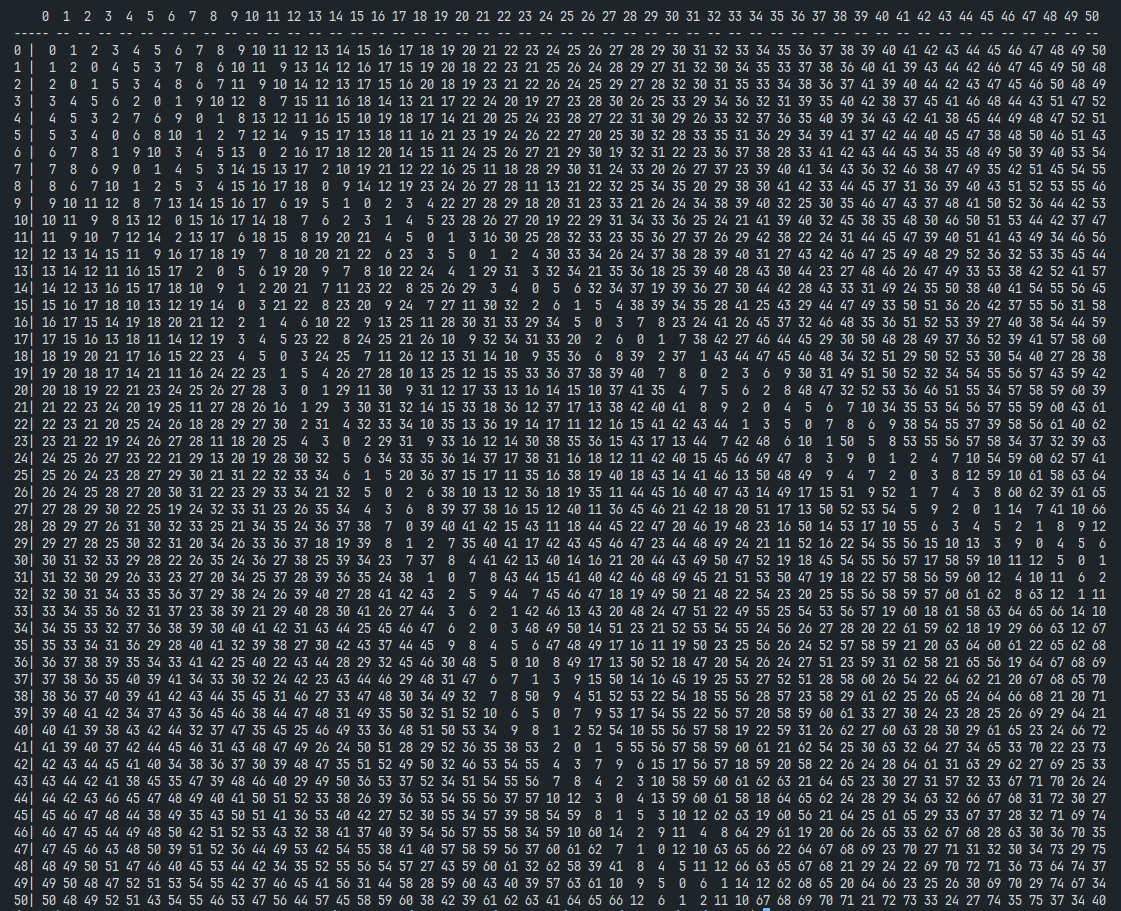
\includegraphics[width=0.8\linewidth]{images/image_output_queen_grundy.png}
  \caption{\(51 \times 51\)のチェス盤のグランディ数}
\end{figure}

さて、このグランディ数を見つめると横軸が\(2\)の列において、周期3、差3の加法周期をなしていることがわかる。
同様に横軸\(3\)の列に着目すると、12列目以降から周期6、差6の加法周期をなしていることが読み取れる。
以上2つより、コーナー・ザ・クイーンは各行にたいして加法周期性を持っていると予想できる。

\begin{thebibliography}{99}
  \bibitem{combination_game_theory} 安福智明, 坂井公, 末續鴻輝. 組み合わせゲーム理論の世界〜数学で解き明かす必勝法〜, 共立出版株式会社, 2024.
\end{thebibliography}

%%%%%%%%%%%%%%%%%%%%%%%%%%%%%%%%%%%%%%%%%%%%%%%%%%%%%%%%%%%%%%%%%%%%%%
\appendix
\setcounter{figure}{0}
\setcounter{table}{0}
\numberwithin{equation}{section}
\renewcommand{\thetable}{\Alph{section}\arabic{table}}
\renewcommand{\thefigure}{\Alph{section}\arabic{figure}}
%\def\thesection{付録\Alph{section}}
\makeatletter 
\newcommand{\section@cntformat}{付録 \thesection:\ }
\makeatother
%%%%%%%%%%%%%%%%%%%%%%%%%%%%%%%%%%%%%%%%%%%%%%%%%%%%%%%%%%%%%%%%%%%%%%

    
\end{document}